\chapter{Termodinámica Química}

\section{Introducción}

La \textbf{Termodinámica} es la parte de la Física que se ocupa del estudio de las relaciones que se establecen entre el calor y el resto de las formas de energía. Entre otras cuestiones la termodinámica se ocupa de analizar los efectos que producen los cambios de magnitudes tales como la temperatura, la densidad, la presión, la masa, el volumen, en los sistemas y a un nivel macroscópico. La base sobre la cual se ciernen todos los estudios de la termodinámica es la circulación de la energía y como ésta es capaz de infundir movimiento. Vale destacar que justamente esta cuestión fue la que promovió el desarrollo de esta ciencia, ya que su origen se debió a la necesidad de aumentar la eficiencia de las primeras máquinas de vapor.\\

Los primeros estudios termodinámicos se deben al ingeniero francés \emph{Nicolas Sadi Carnot (1796-1832)}, quien en 1824 publico un libro titulado \emph{Reflexiones sobre la Fuerza Motriz del Fuego}, donde abordaba la eficiencia de las máquinas de vapor que se utilizaban en la época y los máximos rendimientos que se podían alcanzar con una máquina térmica ideal a la cual se llamó \textbf{Maquina de Carnot}.\\

Las conclusiones obtenidas por Carnot y sus sucesores fueron tan generales y simples que la termodinámica se ha establecido como una disciplina general que se ocupa de describir cómo los sistemas responden a los cambios que se producen en su entorno, pudiéndose aplicar a una infinidad de situaciones tanto de la ciencia como de la ingeniería, como pueden ser: motores, reacciones químicas, transiciones de fase, fenómenos de transporte, agujeros negros… entre otras. 

\section{Termoquímica}

Se define \textbf{Termoquímica} como la parte de la Química que estudia las transferencias energéticas en el transcurso de una reacción química. Dicha energía se manifiesta mayoritariamente en forma de calor, por lo que se puede resumir la termoquímica como la parte de la química que estudia el intercambio calorífico que tiene lugar en una reacción química. Como dicho calor tiene que ver con el contenido de energético de los compuestos químicos intervinientes en el proceso, y teniendo en cuenta que todo sistema químico tiende al estado de mínima energía, la termoquímica se encarga también del estudio de la espontaneidad de las reacciones químicas. 

\section{Sistema Termodinámico}

Se define \textbf{Sistema Termodinámico} como una porción del universo físico que se aísla para su estudio. A la porción del universo físico que se encuentra en contacto con nuestro sistema se le denomina \textbf{Entorno}. Los sistemas termodinámicos se clasifican según el grado de aislamiento que presentan con su entorno. Aplicando este criterio pueden darse tres clases de sistemas:\\

\begin{itemize}
	\item \textbf{Sistema aislado:} Es aquel que no intercambia ni materia ni energía con su entorno, es decir se encuentra en equilibrio termodinámico. Un ejemplo de esta clase podría ser un gas encerrado en un recipiente de paredes rígidas lo suficientemente gruesas (paredes adiabáticas) como para considerar que los intercambios de energía calorífica sean despreciables y que tampoco puede intercambiar energía en forma de trabajo.\\
	
	\item \textbf{Sistema Cerrado:} Es aquel que puede intercambiar energía pero no materia con el exterior. Multitud de sistemas se pueden englobar en esta clase. El mismo planeta Tierra puede considerarse un sistema cerrado. Una lata de sardinas también podría estar incluida en esta clasificación.\\
	
	\item \textbf{Sistema Abierto:} En esta clase se incluyen la mayoría de sistemas que pueden observarse en la vida cotidiana. Por ejemplo, un vehículo motorizado es un sistema abierto, ya que intercambia materia con el exterior cuando es cargado, o su conductor se introduce en su interior para conducirlo, o es provisto de combustible al repostarse, o se consideran los gases que emite por su tubo de escape pero, además, intercambia energía con el entorno. Solo hay que comprobar el calor que desprende el motor y sus inmediaciones o el trabajo que puede efectuar acarreando carga.\\
	
\end{itemize}
	
	Puesto que la gran mayoría de reacciones químicas tienen lugar en disolución, es decir, en un vaso de precipitados, los sistemas químicos se consideran en su mayor parte como \emph{sistemas abiertos}.
	
\section{Variables de Estado}

Una vez determinados los límites de un sistema termodinámico objeto de estudio o investigación, se procede a determinar y cuantificar su estado. En Termodinámica, se denominan \emph{Variables de Estado} a aquellas variables que caracterizan un sistema. Dichas variables son variables macroscópicas, perfectamente medibles en un laboratorio por métodos simples y que caracterizan un estado microscópico concreto. Por ejemplo, en un sistema termodinámico formado por un gas, las variables de estado son la \emph{Presión, Volumen y Temperatura}.\\

Las variables de estado tienen una característica fundamental e importantísima en un proceso: \textbf{Solo dependen de los estados inicial y final del sistema, nunca del proceso seguido}. Esto es de una importancia vital a la hora de estudiar un sistema químico, pues durante una reacción química las variables de estado van a depender exclusivamente de los estados inicial y final, esto es, reactivos y productos, simplificando enormemente el tratamiento teórico de los mismos.

\section{Primer Principio de la Termodinámica}
Pasamos ahora a estudiar el Primer Principio de la Termodinámica que es una generalización del Principio de Conservación de la Energía Mecánica
\subsection{Concepto de Trabajo Termodinámico}

Consideraremos el caso de un gas ideal encerrado en un cilindro con émbolo movil. En cierto momento aumenta la presión en el interior del recipiente y el gas se expande efectuando un trabajo al desplazar el émbolo hacia arriba una longitud infinitamente pequeña (dx). Por tanto, el trabajo efectuado por dicho gas será:

\begin{figure}[h!]
	\centering
	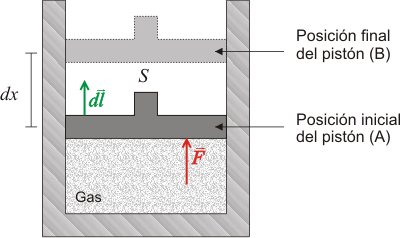
\includegraphics [scale = 0.4]{trabajo1p}
\end{figure}

\begin{definition}[Trabajo Termodinámico]
	Se define en física el trabajo que efectúa una fuerza al desplazar un objeto un elemento dx como:
	\begin{align}
		& W=\int_{x_1}^{x_2}F \cdot dx
	\end{align}
	Sabiendo que $F = P \cdot S$ y que $dV = S \cdot dx$, podemos expresar el trabajo termodinámico en función de las variables de estado de un gas ideal:
	\begin{align}
		& W=\int_{V_1}^{V_2}P \cdot dV
	\end{align}
\end{definition}

Se puede interpretar geométricamente el trabajo como el área encerrada bajo la curva de la gráfica presión-temperatura de un gas ideal.

\begin{figure}[h!]
	\centering
	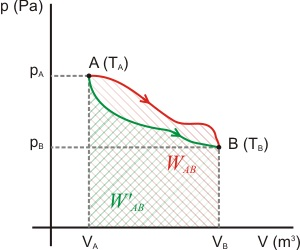
\includegraphics[scale = 0.5]{trabajopV}
\end{figure}

De esta gráfica se puede deducir una consecuencia muy importante. En efecto si analizamos en detalle la gráfica anterior nos daremos cuenta de que el área encerrada bajo la curva es distinta en el proceso de color rojo que en el proceso de color verde, aunque los estados inicial y final de ambos procesos sean los mismos. El Trabajo \emph{no es una función de estado de un sistema termodinámico}.\\

\subsection{Energía Interna}

Se puede entender la \textbf{Energía Interna (U)} en Termodinámica como la medida macroscópica de la energía microscópica de las moléculas que componen un sistema. Se puede considerar como la suma de:\\

\begin{itemize}
	
	\item \textbf{Energía Cinética Interna}, es decir, de las sumas de las energías cinéticas de las individualidades que lo forman respecto al centro de masas del sistema.\\
	
	\item  \textbf{Energía Potencial Interna}, que es la energía potencial asociada a las interacciones entre estas individualidades.\\
	
\end{itemize}

La energía interna no incluye la energía cinética traslacional o rotacional del sistema como un todo. Tampoco incluye la energía potencial que el cuerpo pueda tener por su localización en un campo gravitacional o electrostático externo. Por tanto, es una Energía que no es accesible desde el punto de vista de la mecánica clásica.\\

Como se puede observar, la energía interna solo depende de la configuración macroscópica del sistema, por lo que también es una \emph{función de estado} del mismo. 

\subsection{Criterio de Signos}

Para la formulación del primer principio, debemos de establecer un criterio de signos a la hora de evaluar los intercambios de energía que se producen entre el sistema y el entorno en términos de calor y trabajo. Así, nosotros estableceremos el Criterio Clásico:

\begin{figure}[h!]
	\centering
	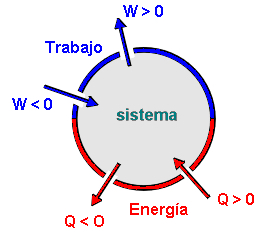
\includegraphics[scale=0.4]{critsignos}
\end{figure}

Como podemos observar el calor que se cede del sistema al entorno lo tomaremos como negativo, mientras que el trabajo que realiza el sistema sobre el entorno lo tomaremos a su vez como positivo.

\subsection{Primer Principio de la Termodinámica}

El primer principio de la Termodinámica qué enunciado en 1850 por \textbf{Clasius} y \textbf{Lord Kelvin}, y es una generalización del Principio de Conservación de la Energía expresado en términos de trabajo y calor. Su enunciado sería:\\

\begin{definition}[Primer Principio de la Termodinámica]
	El aumento de Energía Interna de un Sistema Termodinámico es igual a la diferencia entre el calor aplicado y el trabajo realizado.
	
	\begin{align}
		& \Delta U = Q-W
	\end{align}

O también podemos expresarlo de forma diferencial:\\

	\begin{align}
		& dU = dQ - dW = dQ - PdV
	\end{align}
	
\end{definition}

Para un proceso isocórico (a V=cte.) dV = 0, por lo que se queda:\\

\begin{center}
	$dU = dQ_v$
\end{center}

\begin{definition}[Interpretación de la Energía Interna]
	La Energía Interna de un Sistema Termodinámico se puede interpretar como el calor intercambiado en un proceso a Volumen Constante
\end{definition}

\section{Concepto de Entalpía}

El principal problema que encontramos a la hora de tratar el calor es que éste no es Función de Estado del Sistema. Sería muy interesante encontrar una magnitud calorífica que fuese variable de estado del sistema, pues en el caso de un proceso químico, esta dependería solo del estado final e inicial del proceso, es decir, de los reactivos y productos.\\
\begin{definition}[]
	Se define Entalpía (en griego, “agregar calor”) como:
	\begin{align}
		& H = U + P\cdot V
	\end{align}
\end{definition}

Como podemos observar, U, P y V son variables de estado del sistema, por lo que H también lo es. Si diferenciamos la ecuación obtenemos:\\

\begin{center}
	$dH = dU + PdV + VdP$\\
\end{center}

Despejando el calor del enunciado del Primer Principio:\\

\begin{center}

$dQ = dU + PdV$\\

\end{center}

Como podemos observar, las dos expresiones anteriores son coincidentes en el caso de que hagamos dP = 0, es decir, tengamos un proceso Isobárico (a P = cte). En ese caso se obtiene:\\

\begin{center}
	$dH =dQ_P$\\
\end{center}

Puesto que a mayoría de reacciones químicas se realizan a presión constante (la atmosférica), utilizaremos la entalpía para calcular los calores intercambiados en una reacción química.

\section{Entalpía Estándar de Reacción: Diagramas Entálpicos}

Uno de los factores que más nos interesa estudiar de una reacción química es el de calor que desprende o absorbe un proceso. Según lo visto en el apartado anterior, introducimos el concepto de \emph{Entalpía de Reacción}

\begin{definition}[Entalpía de Reacción]
	
	Se define Entalpía de Reacción $\Delta H_r$ como el calor absorbido o desprendido en una reacción química cuando ésta transcurre a Presión constante
	
\end{definition}

Como los valores de Entalpía de Reacción van a depender de la Presión y la Temperatura, para simplificar los cálculos vamos a definir unas condiciones que tomaremos como referencia a la hora de tabular y de tratar de manera numérica, las denominadas \emph{Condiciones Estándar}\\

\begin{definition}[Condiciones Estándar Termodinámicas]
	Se definen las Condiciones Estándar Termodinámicas como aquellas que corresponden con un Temperatura de 298 K y una Presión de 1 atm.
\end{definition}

Realmente los que conocemos como Entalpía de Reacción es la diferencia de entalpía (incremento) entre reactivos y productos:

\begin{center}
	$\Delta H^{0}_r = H^{0}_{Productos} -  H^{0}_{Reactivos} $
\end{center}

Puesto que la entalpía es una función de estado y además representa al calor de reacción a presión constante (que no olvidemos es energía) las entalpías van a depender del contenido energético de reactivos y productos. Por tanto, en una reacción química nos podemos hallar ante dos situaciones:\\

\begin{itemize}
	\item Que el contenido energético de los productos sea menor que en los reactivos. En ese caso al final de una reacción química habrá un exceso de energía que se transmitirá al entorno en forma de calor. A dicho proceso se le conoce como \textbf{Proceso Exotérmico ($\Delta H^{0}_r < 0$)}\\
	
	\item Que el contenido energético de los productos sea mayor que en los reactivos. En ese caso al final de una reacción química se necesitará un aporte de energía (calor) del medio para que ésta tenga lugar. A dicho proceso se le conoce como \textbf{Proceso Endotérmico ($\Delta H^{0}_r > 0$)}\\
\end{itemize}

Una manera muy útil de ilustrar este proceso es mediante los denominados\emph{Diagramas Entálpicos}:

\begin{figure}[h!]
	\centering
	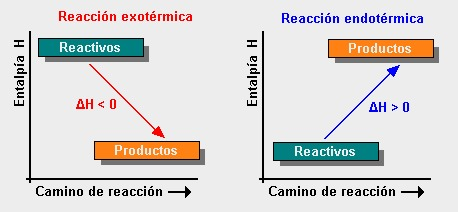
\includegraphics[scale = 0.5]{entalpico}
\end{figure}

Por norma general, se suelen nombrar las entalpías con el nombre del tipo de reacción química presente. Así hablaremos de entalpía de combustión, de hidrólisis, de hidratación…..etc.

\section{Cálculo de Entalpías de Reacción}

En los siguientes apartados estudiaremos los métodos mas utilizados para el cálculo de entalpías de reacción.

\subsection{Entalpías Estándas de Formación}

Se define \textbf{Entalpía Estándar de Formación} como el calor necesario para formar 1 mol de compuesto químico a partir de sus elementos en su estado mas estable (esto es, estado de agregación y forma alotrópica mas estables). Sus unidades en el SI es el J/mol, aunque por su magnitud se suele emplear el KJ/mol.

\begin{center}
	$2C_{(s)Grafito}+2H_{2(g)} \longrightarrow 2C_2H_{2(g)}$ \hspace{1cm} $\Delta H^{0}_f = +54\; KJ/mol$ 
\end{center}

Como en las Entalpías solo podemos calcular sus incrementos y, por tanto, carecemos de una escala absoluta de las mismas, asumiremos por convenio que:\\

\begin{definition}
Las Entalpías de Formación de los Elementos Químicos puros que se hallen en su estado mas estable tienen valor 0.
\end{definition}

Este convenio establecido, y el hecho de que la Entalpía es una función de estado hace que el cálculo de calores de reacción a partir de sus calores de formación sea muy sencillo, puesto que las entalpías de formación de la mayoría de compuestos químicos en condiciones estándar se encuentran tabuladas:

\begin{center}
	$\Delta H^{0}_r = \displaystyle\sum_{i = 1}^{N}(\Delta H^{0}_f)_{Productos} - \displaystyle\sum_{i=1}^{N}(\Delta H^{0}_f)_{Reactivos}$
\end{center}










